\chapter{Программный комплекс}

\section{Непараметрический метод}

\section{Полупараметрический метод}

\section{Выделение компонент связности}



% \subsection{Physics-informed modification of the loss function}
% \label{section_informed_methodology}


% \new{The proposed physics-informed approach involves modifying the standard loss function, that is:
	% \begin{equation*}
		%     Loss(y_{true}, y_{predict})[i] = (1-\alpha) \cdot MSE(y_{true}, y_{predict})[i] + \alpha(t) \cdot (y_{predict} - A[i] - \sum_{j=1}^3 B_{ij} e_{ij})^2,
		% \end{equation*}
	% where $i\in \{1, 2, 3\}$ represents the variable index ($0$ for cumulative flux, $1$ for SST and $2$ for pressure),
	% \begin{equation*}
		% MSE=\frac1n\sum\limits_{j=1}n \left(y_{true}-y_{predict}\right)^2 
		% \end{equation*}
	% stands for standard mean squared error, $A_[i]$ are the estimates of the drift coefficient, $B_{ij}$ and $e_{ij}$,  $j \in \{1, 2, 3\}$ are the obtained estimations of the first eigenvalues and eigenvectors from the ordered set, and $\alpha(t)$ is the weight coefficient, that can be either a kind of hyperparameter or the self-adapting~\citep{Xiang2022} part of a neural network.
	% % , vanishing with each epoch number of the additional steps $t \in \{0, 1, \dots, 10\}$:
	% % $$
	% %     \alpha(t) = 0.6 \cdot 0.9^{-t}.
	% % $$
	% This modified loss function implements a variant of stochastic regularization to prevent the model from violating predictions, allowing neural networks to adjust to SDE limitations, and this can increase forecast quality.
	% }

\section{Архитектура программного обеспечения}

В этом разделе мы кратко опишем архитектуру программного обеспечения. Предварительная и последующая обработка данных может выполняться как в рамках серверного решения, так и на одном ПК (см. уровень "Единой системы" на рисунке~\ref{algorithm_pic}). Однако обработка пространственно-временных данных на основе процедуры, описанной в подразделе~\ref{Sec Karhunen}, требует больше вычислительных ресурсов. Итак, повторный анализ данных за 46 лет был проведен на кластере (см. уровень "Компьютерный кластер" на рисунке~\ref{algorithm_pic}). Схема декомпозиции Карунена-Лоэева представлена в нижней части рисунка ~\ref{algorithm_pic}. 


\begin{figure}
	\center{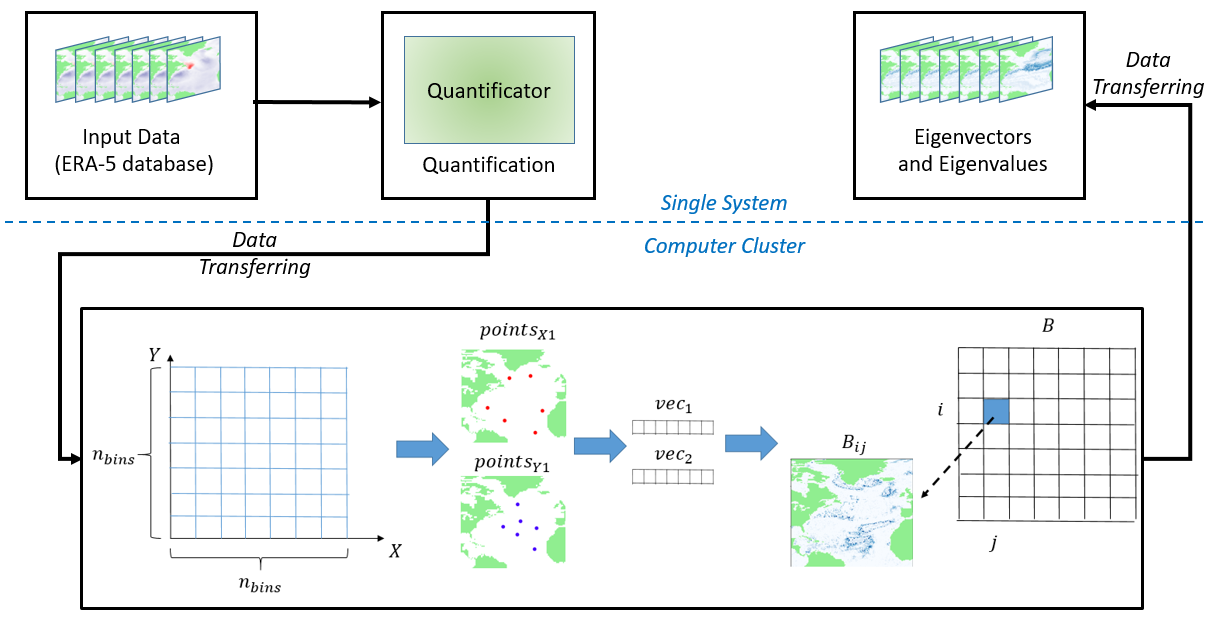
\includegraphics[width=\textwidth]{eigenvalues_algo.png}}
	\caption{Архитектура программного обеспечения}
	\label{algorithm_pic}
\end{figure}


